% Create a document for a project proposal
\documentclass[10pt]{article}
% Packages
\usepackage{geometry}
\geometry{
    top=1.5cm,
    bottom=1.5cm,
    left=2cm,
    right=2cm
}
\usepackage{ragged2e}
\usepackage{algorithm}
\usepackage{algpseudocode}
\usepackage{graphicx}
% Options for packages loaded elsewhere
\PassOptionsToPackage{unicode}{hyperref}
\PassOptionsToPackage{hyphens}{url}
\usepackage{amsmath,amssymb}
\usepackage{lmodern}
\usepackage{iftex}
\ifPDFTeX
  \usepackage[T1]{fontenc}
  \usepackage[utf8]{inputenc}
  \usepackage{textcomp} % provide euro and other symbols
\else % if luatex or xetex
  \usepackage{unicode-math}
  \defaultfontfeatures{Scale=MatchLowercase}
  \defaultfontfeatures[\rmfamily]{Ligatures=TeX,Scale=1}
\fi
% Use upquote if available, for straight quotes in verbatim environments
\IfFileExists{upquote.sty}{\usepackage{upquote}}{}
\IfFileExists{microtype.sty}{% use microtype if available
  \usepackage[]{microtype}
  \UseMicrotypeSet[protrusion]{basicmath} % disable protrusion for tt fonts
}{}
\makeatletter
\@ifundefined{KOMAClassName}{% if non-KOMA class
  \IfFileExists{parskip.sty}{%
    \usepackage{parskip}
  }{% else
    \setlength{\parindent}{0pt}
    \setlength{\parskip}{6pt plus 2pt minus 1pt}}
}{% if KOMA class
  \KOMAoptions{parskip=half}}
\makeatother
\usepackage{xcolor}
\setlength{\emergencystretch}{3em} % prevent overfull lines
\providecommand{\tightlist}{%
  \setlength{\itemsep}{0pt}\setlength{\parskip}{0pt}}
\setcounter{secnumdepth}{-\maxdimen} % remove section numbering
\newlength{\cslhangindent}
\setlength{\cslhangindent}{1.5em}
\newlength{\csllabelwidth}
\setlength{\csllabelwidth}{3em}
\newlength{\cslentryspacingunit} % times entry-spacing
\setlength{\cslentryspacingunit}{\parskip}
\newenvironment{CSLReferences}[2] % #1 hanging-ident, #2 entry spacing
 {% don't indent paragraphs
  \setlength{\parindent}{0pt}
  % turn on hanging indent if param 1 is 1
  \ifodd #1
  \let\oldpar\par
  \def\par{\hangindent=\cslhangindent\oldpar}
  \fi
  % set entry spacing
  \setlength{\parskip}{#2\cslentryspacingunit}
 }%
 {}
\usepackage{calc}
\newcommand{\CSLBlock}[1]{#1\hfill\break}
\newcommand{\CSLLeftMargin}[1]{\parbox[t]{\csllabelwidth}{#1}}
\newcommand{\CSLRightInline}[1]{\parbox[t]{\linewidth - \csllabelwidth}{#1}\break}
\newcommand{\CSLIndent}[1]{\hspace{\cslhangindent}#1}
\ifLuaTeX
  \usepackage{selnolig}  % disable illegal ligatures
\fi
\IfFileExists{bookmark.sty}{\usepackage{bookmark}}{\usepackage{hyperref}}
\IfFileExists{xurl.sty}{\usepackage{xurl}}{} % add URL line breaks if available
\urlstyle{same} % disable monospaced font for URLs
\hypersetup{
  hidelinks,
  pdfcreator={LaTeX via pandoc}}

% Title
\title{\textbf{Design \& Analysis of Algorithms Report \\ \vspace{5mm} EEG classification using Deep Learning Algorithms}}
\author{\textbf{Team Members} \vspace{1mm} \\ Muhammad Athar (408369) \\ Muhammad Arsalan Khan (410963) \vspace{5mm} \\ \textbf{Class: }BESE - 13A}

\begin{document}
\maketitle

\tableofcontents
\newpage

\justifying
\section{Introduction}
The semester project for Design and Analysis of Algorithms aims to tackle the problem of classifying EEG (Electroencephalography) files as either normal or abnormal.
Electroencephalography (EEG) is a non-invasive method used to record electrical activity of the brain. However, manual analysis of EEG data is time consuming and requires expertise of highly trained neurologists. Unfortunately, there is a lack of clinically certified neurologists in developing countries especially in Pakistan. Therefore, the aim of this project is to develop a deep learning model that can classify EEG files as either normal or abnormal. Such deep learning model would help in the initial screening of EEG files and would reduce the workload of neurologists.

\subsection{Selection of Algorithm}
For the classification of EEG recordings, we have looked into many architectures like ResNet 18 and Temporal Networks, but among them, SCNet seems to give the best results according to literature. So we have decided to implement this architecture for this task. The model will be trained on the TUH EEG Corpus, taken from Temple University, which is one of the largest publicly available dataset of EEG Recordings.

\subsection{Steps}
The project will be divided into the following steps:
\begin{enumerate}
    \item Data Collection: Collect EEG files from the TUH EEG Corpus.
    \item Data Preprocessing: Preprocess the EEG files to get the required format.
    \item Feature Extraction: Extract features from the EEG files.
    \item Model Training: Train the model using the extracted features.
    \item Model Evaluation: Evaluate the model using various metrics like accuracy.
\end{enumerate}

\section{Contributions} 
\subsection{Algorithm} 
\begin{enumerate}
  \item The first step of the algorithm involves preprocessing the raw EEG recordings to make them suitable for training. The preprocessing steps involve:
  \begin{itemize}
    \item Selection of 21 standard channels that exist in all EEG recordings.
    \item Downsampling the EEG recordings to 100 Hz.
    \item Clipping the absolute amplitude between the range 0 to 100 $\mu$V.
    \item Taking the part of the recording from the start of 1st minute to the end of the 7th minute.
  \end{itemize}
  \item The second step of the algorithm involves extracting spatial features from the preprocessed EEG recordings. It is done so by taking the average, maximum, and standard deviation across all channels, and appending them to the feature vector. At this point, the shape of the training data is (24, length of recording).
  \item The third step of the algorithm involves extracting temporal features. By using multiple 1D convolutional layers inside Multi-feature fusion modules(MFFM). The MFFM uses skip connections between two consecutive convolutional layers for the fusion of characteristics from different network layers.
  \item After passing through all these convolutional layers, the output is passed through a global average pooling layer and a softmax layer is applied to get the final output.
  \item The model is trained using the Adam optimizer with a learning rate of 1e-3 and a batch size of 32. The model is trained for 60 epochs.
\end{enumerate}

\subsection{Equations}
\[ s_{gap}^t = \frac{1}{C} \sum_{c=1}^{C} x_{ct} \]
Above equation is used to calculate the average of the EEG data across all channels at time t.

\[ s_{gmp}^t = max\{x_{ct}\} \]
Above equation is used to calculate the maximum value of the EEG data across all channels at time t.

\[ s_{gsp}^t = \frac{1}{C} \sqrt{\sum_{c=1}^{C} (x_{ct} - s_{gap}^t)^2} \]
Above equation is used to calculate the standard deviation of the EEG data across all channels at time t.
\newline
All the above equations are used to calculate values for all times t=1,2,...,T. C = 21 is the number of channels selected.

\subsection{Diagrams}
\begin{figure}[H]
    \centering
    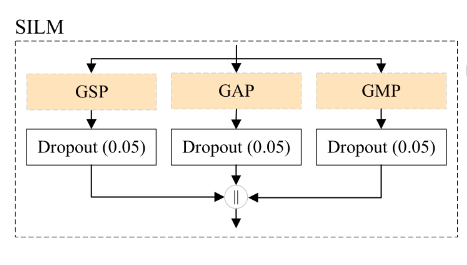
\includegraphics[width=0.7\textwidth]{silm.png}
    \caption{Spatial Information Learning Module (SILM)}
    \label{fig:silm}
\end{figure}
Figure \ref{fig:silm} shows that SILM applies GSP(Global standard deviation Pooling), GAP(Global Average Pooling), and GMP(Global Max Pooling) across all channels, followed by a dropout layer of 0.05 on each. They are then concatenated.

\begin{figure}[H]
    \centering
    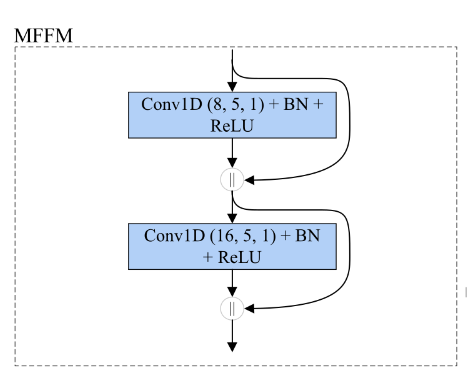
\includegraphics[width=0.4\textwidth]{mffm.png}
    \caption{Multi-feature Fusion Module (MFFM)}
    \label{fig:mffm}
\end{figure}
Figure \ref{fig:mffm} shows that the MFFM involves two consecutive 1D convolutional layers, followed by Batch Normalization and ReLU activation function on each. Before applying the next convolutional layer, the output of the previous layer is concatenated.

\begin{figure}[H]
    \centering
    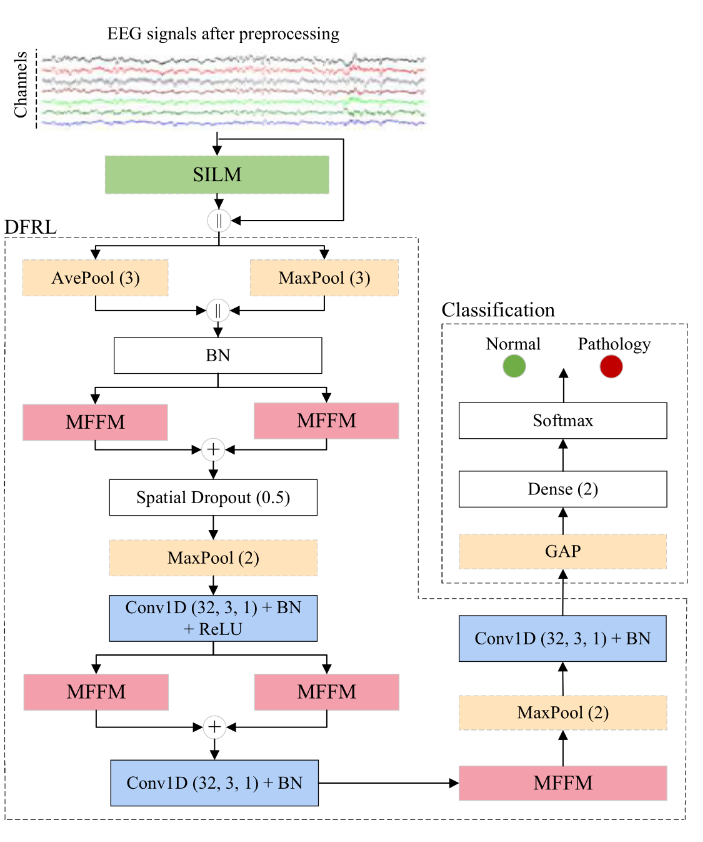
\includegraphics[width=0.59\textwidth]{model.png}
    \caption{SCNet Architecture}
    \label{fig:model}
\end{figure}
Figure \ref{fig:model} shows that the entire SCNet architecture, with Average and Max Pooling in between layers, to reduce the input dimensions at each stage. At the end, a softmax classifier is used to classify the EEG data.

\subsection{Pseudocodes}

\begin{algorithm}[H]
  \caption{Preprocessing}
      \begin{algorithmic}[1]
      \Procedure{Preprocess}{Raw EEG} \Comment{The Raw EEG is input}
          \State Total Channels $\gets 21$
          \State Input Format: Raw EEG Data
          \State 
          \State Output Format: Preprocessed EEG Data
          \State
  
          \State Output $\gets$ \Call{selectChannels}{Raw EEG, 21} \Comment{Select 21 Standard channels}
          \State Output $\gets$ \Call{downsample}{Output, 100 Hz} \Comment{Downsample to 100 Hz}
          \State Output $\gets$ \Call{clipAmplitude}{Output, 0, 100 $\mu$V} \Comment{Clip amplitude between 0 to 100 $\mu$V}
          \State Output $\gets$ \Call{selectTime}{Output, 1st to 8th minute} \Comment{Select 1st minute to 8th minute}
          \State \textbf{return} Output \Comment{Returns the preprocessed data} 
      \EndProcedure
      \end{algorithmic}
  \end{algorithm}

\begin{algorithm}[H]
\caption{SILM}
    \begin{algorithmic}[2]
    \Procedure{Classify}{Preprocessed EEG} \Comment{The preprocessed EEG is input}
        \State Total Channels $\gets 21$
        \State Input Format: EEG data $[e_{ij}]$ where $i \gets 1$ to $21$ where 21 is the number of channels
        \State and $j \gets 1$ to $n$ where $n$ is the number of timestamps
        \State 
        \State Output Format: The EEG data with concatenated GAP, GMP, and GSP
        \State

        \State GAP out $\gets$ \Call{GAP}{Preprocessed EEG} \Comment{Global Average Pooling}
        \State GMP out $\gets$ \Call{GMP}{Preprocessed EEG} \Comment{Global Max Pooling}
        \State GSP out $\gets$ \Call{GSP}{Preprocessed EEG} \Comment{Global Standard Deviation Pooling}
        \State Preprocessed EEG $\gets$ \Call{Concat}{Preprocessed EEG, GAP out, GMP out, GSP out} \Comment{Concatenate the outputs}
        \State \textbf{return} Preprocessed EEG \Comment{Returns the preprocessed EEG with concatenated features}
    \EndProcedure
    \end{algorithmic}
\end{algorithm}

\begin{algorithm}[H]
  \caption{1D Convolutional Layer}
  \begin{algorithmic}[3]
      \Procedure{Conv1D}{data, kernel, stride}
      \State Input Format: $[e_{ik}]$ where $i \gets 0$ to $h_0$ and $k \gets 0$ to $w_0$
      \State Output Format: $[o_{ij}]$ where $i \gets 0$ to $h_0$, $j \gets 0$ to $w_1$

      \Comment The height of the data remains the same
      \State $w_0 \gets width$, $h_0 \gets height$
      \State $w_1 \gets \frac{w_0 - kernel}{stride} + 1$  \Comment Calculate the width of the output
      \State for $i \gets 0$ to $h_0$ do
      \State \hspace{1cm} for $j \gets 0$ to $w_1$ do
      \State \hspace{2cm} $[o_{ij}] \gets \sum_{k=j*stride}^{j*stride + kernel} [w_{ik}] * [e_{ik}] + b$ \Comment{Slide the kernel through input data}
      \State \hspace{1cm} end for
      \State end for

      \State \textbf{return} $[o_{ij}]$
      \EndProcedure
  \end{algorithmic}
\end{algorithm}

\begin{algorithm}[H]
\caption{ReLU Activation Function}
    \begin{algorithmic}[4]
    \Procedure{ReLU}{data} 
          \State Input Format: $[e_{ij}]$ where $i \gets 0$ to $h$ and $j \gets 0$ to $w$
          \State 
          \State Output Format: $[o_{ij}]$ where $i \gets 0$ to $h$ and $j \gets 0$ to $w$
          \State
          \State for $i \gets 0$ to $h$ do
          \State \hspace{1cm} for $j \gets 0$ to $w$ do
          \State \hspace{2cm} $[o_{ij}] \gets max(0, [e_{ij}])$ \Comment{Apply ReLU activation function}
          \State \hspace{1cm} end for
          \State end for
          \State \textbf{return} $[o_{ij}]$ \Comment{Returns the output after applying ReLU}
    \EndProcedure
    \end{algorithmic}
    
\end{algorithm}

\begin{algorithm}[H]
  \caption{Batch Normalization}
      \begin{algorithmic}[4]
      \Procedure{BatchNorm}{data} 
          \State Input Format: $[e_{ij}]$ where $i \gets 0$ to $h$ and $j \gets 0$ to $w$
          \State
          \State Output Format: $[o_{ij}]$ where $i \gets 0$ to $h$ and $j \gets 0$ to $w$
          \State
          \State $\mu \gets \frac{1}{h*w} \sum_{i=0}^{h} \sum_{j=0}^{w} [e_{ij}]$ \Comment{Calculate the mean}
          \State $\sigma^2 \gets \frac{1}{h*w} \sum_{i=0}^{h} \sum_{j=0}^{w} ([e_{ij}] - \mu)^2$ \Comment{Calculate the variance}
          \State $[o_{ij}] \gets \frac{[e_{ij}] - \mu}{\sqrt{\sigma^2 + \epsilon}}$ \Comment{Normalize the data}
          \State \textbf{return} $[o_{ij}]$ \Comment{Returns the output after applying Batch Normalization}
      \EndProcedure
      \end{algorithmic}
      
  \end{algorithm}


  \begin{algorithm}[H]
    \caption{Multi-feature Fusion Module}
        \begin{algorithmic}[5]
        \Procedure{MFFM}{data} \Comment{The Raw EEG is input}
            \State Input Format: $[e_{ij}]$ where $i \gets 0$ to $h$ and $j \gets 0$ to $w$
            \State
            \State Output Format: $[o_{ij}]$ where $i \gets 0$ to $h$ and $j \gets 0$ to $w$
            \State
            \State x1 $\gets$ \Call{Conv1D}{data, 8, 5} \Comment{Apply 1D Convolutional Layer}
            \State x1 $\gets$ \Call{BatchNorm}{x1} \Comment{Apply Batch Normalization}
            \State x1 $\gets$ \Call{ReLU}{x1} \Comment{Apply ReLU Activation Function}
            \State x2 $\gets$ \Call{Concat}{x1, data} \Comment{Concatenate the output with the input}
            \State x2 $\gets$ \Call{Conv1D}{x2, 16, 5} \Comment{Apply 1D Convolutional Layer}
            \State x2 $\gets$ \Call{BatchNorm}{x2} \Comment{Apply Batch Normalization}
            \State x2 $\gets$ \Call{ReLU}{x2} \Comment{Apply ReLU Activation Function}
            \State Output $\gets$ \Call{Concat}{data, x1, x2} \Comment{Concatenate the result at all three stages}
            \State \textbf{return} Output \Comment{Returns the output}
        \EndProcedure
        \end{algorithmic}
        
    \end{algorithm}

    \begin{algorithm}[H]
      \caption{Softmax Layer}
          \begin{algorithmic}[7]
          \Procedure{Softmax}{data} 
              \State Input Format: $[e_{i}]$ where $i \gets 0$ to $num\_classes$
              \State
              \State Output Format: $[o_{i}]$ where $i \gets 0$ to $num\_classe$
              \State
              \State for $i \gets 0$ to $num\_classes$ do
              \State \hspace{1cm} $Output_i$ $\gets \frac{e^{[data_{i}]}}{\sum_{j=0}^{num\_classes} e^{[data_{j}]}}$ \Comment{Apply Softmax}
              \State \textbf{return} Output \Comment{Returns the output after applying Softmax}
          \EndProcedure
          \end{algorithmic}
          
      \end{algorithm}

      \begin{algorithm}[H]
        \caption{SCNet Architecture}
            \begin{algorithmic}[8]
            \Procedure{SCNet}{Preprocessed EEG}
                \State Total Channels $\gets 21$
                \State Input Format: EEG data Channels $[e_i]$ where $i \gets 0$ to $21$
                \State $e_i \gets [e_j]$ where $j \gets 0$ to $n$ where $n$ is the number of timestamps
                \State 
                \State Output Format: Class of the EEG in binary (Abnormal/Normal)
                \State
                \State x $\gets$ \Call{SILM}{Preprocessed EEG} \Comment{Apply SILM}
                \State x1 $\gets$ \Call{AvgPool}{x, 3} \Comment{AvgPool with stride 3}
                \State x2 $\gets$ \Call{MaxPool}{x, 3}  \Comment{MaxPool with stride 3}
                \State x $\gets$ \Call{Concat}{x1, x2} \Comment{Concatenate the outputs}
                \State x $\gets$ \Call{BatchNorm}{x} \Comment{Apply Batch Normalization}
                \State x1 $\gets$ \Call{MFFM}{x} \Comment{Apply MFFM}
                \State x2 $\gets$ \Call{MFFM}{x} \Comment{Apply MFFM}
                \State x $\gets$ \Call{SpatialDropout}{x1 + x2, 0.5} \Comment{Apply Spatial Dropout}
                \State x $\gets$ \Call{MaxPool}{x, 2} \Comment{MaxPool with stride 2}
                \State x $\gets$ \Call{Conv1D}{x, 32, 3}
                \State x $\gets$ \Call{BatchNorm}{x} \Comment{Apply Batch Normalization}
                \State x $\gets$ \Call{ReLU}{x} \Comment{Apply ReLU Activation Function}
                \State x1 $\gets$ \Call{MFFM}{x} \Comment{Apply MFFM}
                \State x2 $\gets$ \Call{MFFM}{x} \Comment{Apply MFFM}
                \State x $\gets$ \Call{Conv1D}{x1 + x2, 32, 3}
                \State x $\gets$ \Call{BatchNorm}{x} \Comment{Apply Batch Normalization}
                \State x $\gets$ \Call{MFFM}{x} \Comment{Apply ReLU Activation Function}
                \State x $\gets$ \Call{MaxPool}{x, 2} \Comment{MaxPool with stride 2}
                \State x $\gets$ \Call{Conv1D}{x, 32, 3}
                \State x $\gets$ \Call{BatchNorm}{x} \Comment{Apply Batch Normalization}
                \State x $\gets$ \Call{GAP}{x} \Comment{Apply Global Average Pooling}
                \State x $\gets$ \Call{Dense}{x, 2}
                \State x $\gets$ \Call{Softmax}{x} \Comment{Apply Softmax}
            \EndProcedure
            \end{algorithmic}
            
        \end{algorithm}

\subsection{Problems Encountered}
One of the main problem we encountered is in the training of the model. Even after obtaining computational resources, the dataset (TUH EEG Corpus) was still very large (About 50 GB) which can't be loaded into the RAM all at once and trained on. For this we started preprocessing the data and storing it in tf records. This helped in training the model by loading the data on the fly.
However, even after we trained the model, we encountered another setback, which was that we were uanble to get a good performance on the evaluation set, even though it was giving accuracies upto 99\% on the training data(which should not be possible). The accuracy on the evaluation set never went above 50\%. It could be that the model is unable to generalize to the evaluation set. We are still trying to resolve this issue till date.


\section{Conclusion}
In conclusion, the SCNet model has been chosen for the classification of EEG files as it has shown to be effective in classifying EEG files into normal and abnormal. The model is light-weight and has a high accuracy of 90.57\%. (Wu et al., 2023)

\section{References}
\hypertarget{refs}{}
\begin{CSLReferences}{1}{0}
\leavevmode\vadjust pre{\hypertarget{ref-WU2023105059}{}}%
Wu, Tao, Yujie Fan, Yunning Zhong, Xiu Cheng, Xiangzeng Kong, and Lifei
Chen. 2023. {``SCNet: A Spatial Feature Fused Convolutional Network for
Multi-Channel EEG Pathology Detection.''} \emph{Biomedical Signal
Processing and Control} 86: 105059.
\url{https://doi.org/10.1016/j.bspc.2023.105059}.

\end{CSLReferences}

\vspace{0.5cm}
\hypertarget{refs}{}
\begin{CSLReferences}{1}{0}
\leavevmode\vadjust pre{\hypertarget{ref-he2015deep}{}}%
He, Kaiming, Xiangyu Zhang, Shaoqing Ren, and Jian Sun. 2015. {``Deep
Residual Learning for Image Recognition.''}
\url{https://arxiv.org/abs/1512.03385}.

\end{CSLReferences}

\vspace{0.5cm}
\begin{CSLReferences}{1}{0}
\leavevmode\vadjust pre{\hypertarget{ref-schirrmeister2017deep}{}}%
Schirrmeister RT, Springenberg JT, Fiederer LDJ, Glasstetter M, Eggensperger K, Tangermann M, Hutter F, Burgard W, Ball T. {``Deep learning with convolutional neural networks for EEG decoding and visualization.''} Hum Brain Mapp. 2017 Nov;38(11):5391-5420. doi: 10.1002/hbm.23730. Epub 2017 Aug 7. PMID: 28782865; PMCID: PMC5655781.
\url{}
\end{CSLReferences}

\end{document}